\documentclass[11pt]{article}
\usepackage[review]{acl}
\usepackage{times}
\usepackage{latexsym}
\usepackage[T1]{fontenc}
\usepackage[utf8]{inputenc}
\usepackage{microtype}
\usepackage{inconsolata}
\usepackage{graphicx}
\usepackage{booktabs}
\usepackage{capt-of}
\usepackage[indonesian]{babel}
\usepackage{xurl}

\title{StereoQueerEval: Klasifikasi Ujaran Kebencian terhadap\
Komunitas LGBTQIA+ dengan XLM-RoBERTa dan Qwen3.5-9B}
\author{Penulis Anonim}

\begin{document}
\nolinenumbers
\raggedbottom
\maketitle
\begin{abstract}
% Evidence: Q001,Q002,Q004,B002.
Penelitian ini menyajikan penyelesaian Subtask B StereoQueerEval melalui klasifikasi komentar YouTube berbahasa Inggris, Italia, dan Belanda ke dalam kelas \texttt{no}, \texttt{yes\_implicit}, dan \texttt{yes\_explicit}. Pendekatan utama menyesuaikan Qwen3.5-9B dengan LoRA, menggunakan tiga pilihan bahasa \textit{prompt}. XLM-RoBERTa Base digunakan sebagai pembanding pada pembagian data yang sama. Seluruh pilihan \textit{prompt} Qwen menghasilkan \textit{macro-F1} lebih tinggi daripada pembanding. Skor tertinggi pada pengujian internal adalah 0,719146 pada data Inggris, 0,7036 pada data Italia, dan 0,641522 pada data Belanda. Kesamaan bahasa \textit{prompt} dan komentar belum memberikan hasil tertinggi secara konsisten. Kelas \texttt{yes\_implicit} memperoleh F1 terendah pada kedua model.
\end{abstract}

\section{Pendahuluan}
% Evidence: L102.
Deteksi \textit{hate speech} tidak hanya berkaitan dengan pengenalan kata-kata kasar. Pesan yang menyerang kelompok tertentu juga dapat disampaikan melalui ungkapan tersirat yang membutuhkan pemahaman konteks. \citet{elsherief-etal-2021-latent} menjelaskan bahwa bahasa berkode dan ungkapan tidak langsung menjadi tantangan dalam mendeteksi pesan tersebut. Perbedaan cara penyampaian membuat model perlu mengenali maksud pesan, bukan hanya kata-kata yang muncul di dalamnya.

% Evidence: L111.
Penelitian \citet{chan-etal-2024-hate} mengkaji deteksi \textit{hate speech} terhadap komunitas LGBTQIA+ menggunakan GPT-3.5-turbo pada teks asli dan teks yang diterjemahkan ke bahasa Inggris. Penerjemahan tidak selalu membantu klasifikasi. Analisis kesalahan menunjukkan bahwa istilah \textit{slang} dan ungkapan yang berkaitan dengan budaya tertentu tidak diterjemahkan dengan tepat. Hasil ini menjadi pertimbangan untuk mempertahankan bahasa asli komentar.

% Evidence: L111,Q001,Q006.
Salah satu hal yang belum diuji oleh \citet{chan-etal-2024-hate} adalah penggunaan bahasa \textit{prompt} yang berbeda. Penelitian tersebut menggunakan \textit{prompt} berbahasa Inggris, termasuk untuk data non-Inggris, dan menyarankan pengujian bahasa \textit{prompt} yang sesuai dengan data beserta model lain. Saran ini menjadi dasar penggunaan Qwen dengan \textit{prompt} Inggris, Italia, dan Belanda, baik pada bahasa komentar yang sama maupun berbeda.

% Evidence: L110,L115,Q001,B002.
Penelitian ini berfokus pada penyelesaian \textit{Subtask B: Hate Speech Classification} dalam SemEval-2027 Task 8: StereoQueerEval. Komentar berbahasa Inggris, Italia, dan Belanda diklasifikasikan ke dalam kelas \texttt{no}, \texttt{yes\_implicit}, dan \texttt{yes\_explicit}. XLM-RoBERTa digunakan sebagai \textit{baseline} karena prapelatihan multibahasanya mendukung berbagai tugas pemahaman bahasa lintas bahasa \citep{conneau-etal-2020-unsupervised}. Hasilnya dibandingkan dengan Qwen pada \textit{test} yang sama.

% Evidence: Q001,Q002,Q004,Q006,B002.
Tujuan penelitian ini adalah menyelesaikan klasifikasi dengan membandingkan XLM-RoBERTa dan Qwen melalui sembilan kombinasi bahasa data dan bahasa \textit{prompt}. Tiga versi \textit{prompt} memuat arahan dengan makna yang setara, sementara komentar tetap menggunakan bahasa aslinya. Hasil dianalisis untuk melihat apakah kesamaan bahasa \textit{prompt} dan komentar memberikan skor lebih tinggi, sekaligus mengenali kelas yang masih sulit dibedakan.

\section{Deskripsi \textit{Task}}
% Evidence: L110,L117,Q001.
SemEval-2027 Task 8: StereoQueerEval mengkaji stereotip dan ujaran kebencian terhadap komunitas LGBTQIA+.\footnote{\url{https://semeval.github.io/SemEval2027/tasks.html}} Subtask B meminta klasifikasi komentar ke dalam tiga kelas: \texttt{no} untuk komentar tanpa ujaran kebencian, \nolinkurl{yes_implicit} untuk kebencian yang disampaikan tidak langsung, dan \nolinkurl{yes_explicit} untuk kebencian yang dinyatakan langsung \citep{stereoqueereval-2026-data}. Percobaan menggunakan bahasa Inggris (EN), Italia (IT), dan Belanda (NL). Teks komentar menjadi \textit{input} model, tanpa judul, deskripsi video, atau anotasi dari \textit{subtask} lain.

\section{Metodologi}
\subsection{Model}
% Evidence: L115.
XLM-RoBERTa adalah model \textit{Transformer} multibahasa dengan arsitektur \textit{encoder}. Prapelatihannya menggunakan lebih dari 2 TB teks dari 100 bahasa melalui \textit{masked language modeling}, yaitu memprediksi token yang disembunyikan berdasarkan konteksnya \citep{conneau-etal-2020-unsupervised}. Varian Base selanjutnya disebut XLM-R.

% Evidence: L103.
Qwen3.5-9B merupakan model multibahasa dengan sekitar sembilan miliar parameter \citep{qwen-team-2026-qwen35}. Komponen bahasanya memperkirakan token berikutnya berdasarkan konteks sebelumnya. Model dapat menghasilkan \textit{output} teks sesuai \textit{prompt} dalam format percakapan.

\subsection{Alur Analisis}
\subsubsection{Eksplorasi Data (EDA)}
% Evidence: Q007.
Eksplorasi data atau \textit{exploratory data analysis} (EDA) memeriksa distribusi kelas, kelengkapan kolom, keunikan ID, dan duplikasi. Hasil pemeriksaan digunakan untuk memahami komposisi data sebelum pembagian.

\subsubsection{Prapemrosesan dan Pembagian Data}
% Evidence: Q005,Q007,L118.
Prapemrosesan menggunakan normalisasi Unicode NFKC untuk menyeragamkan representasi karakter yang setara agar kesamaan teks dapat diperiksa secara konsisten \citep{unicode-consortium-2026-normalization}. Kapitalisasi, emoji, dan tanda baca dipertahankan. Komentar tidak diterjemahkan.

% Evidence: Q005,Q007,Q001,B002.
Pembagian dilakukan per bahasa dengan stratifikasi label dan pengelompokan konteks video, menggunakan \textit{seed} 42. Targetnya 70\% \textit{train}, 10\% \textit{validation}, dan 20\% \textit{test}. Komentar dengan pasangan judul--deskripsi yang sama atau duplikat setelah normalisasi ditempatkan pada kelompok yang sama agar tidak terpisah antarbagian. Komentar kemudian ditokenisasi dan dipotong sesuai batas \textit{input} masing-masing model.

\subsubsection{Pelatihan dan Prediksi}
% Evidence: B002.
XLM-R menggunakan lapisan klasifikasi untuk menghasilkan satu dari tiga label. Seluruh parameter diperbarui selama pelatihan. Bobot kelas dihitung hanya dari \textit{train} untuk memperhatikan kelas dengan contoh lebih sedikit.

% Evidence: Q001,Q004,L104.
Penyesuaian Qwen menggunakan \textit{Low-Rank Adaptation} (LoRA) dan \textit{supervised fine-tuning} (SFT). LoRA mempertahankan bobot utama model dan memperbarui parameter tambahan berukuran kecil \citep{hu-etal-2021-lora}. Perhitungan kesalahan hanya dilakukan pada bagian \textit{output}, tanpa menyertakan \textit{prompt} dan komentar.

% Evidence: Q001,Q004,Q006.
\textit{Prompt} menjelaskan tiga kategori dan menegaskan bahwa penyebutan identitas LGBTQIA+ saja tidak cukup untuk menentukan kebencian. Pilihan bahasanya adalah Inggris, Italia, dan Belanda, tanpa contoh komentar berlabel. \textit{Output} dipetakan menjadi angka 0 untuk \texttt{no}, 1 untuk \texttt{yes\_explicit}, dan 2 untuk \texttt{yes\_implicit}. Saat prediksi, jumlah log probabilitas setiap pilihan beserta penanda akhirnya dihitung. Pilihan dengan skor tertinggi menjadi label prediksi.

\subsubsection{Evaluasi Model}
% Evidence: Q001,Q003,Q004,B002.
Evaluasi pada akhir setiap \textit{epoch} digunakan untuk memilih model dengan \textit{macro-F1} tertinggi pada \textit{validation}. Model terpilih dievaluasi pada \textit{test} yang sama untuk kedua pendekatan. Label yang benar pada \textit{test} hanya digunakan untuk menghitung metrik evaluasi.

\subsection{Metrik Evaluasi}
% Evidence: Q001,Q003,Q004,B002.
Metrik utama adalah \textit{macro-F1}, yaitu rata-rata F1 ketiga kelas dengan bobot yang sama. F1 menggabungkan \textit{precision}, yaitu proporsi prediksi suatu kelas yang benar, dan \textit{recall}, yaitu proporsi contoh kelas tersebut yang berhasil dikenali. F1 setiap kelas juga dilaporkan untuk menilai kategori yang lebih sulit dikenali.

\section{Rancangan Eksperimen}
% Evidence: Q005,Q007,L110.
\textit{Dataset} terdiri atas 7.627 komentar berlabel dari penyelenggara StereoQueerEval. Pengujian menggunakan pembagian internal data tersebut, sehingga hasil belum merupakan evaluasi resmi \textit{shared task}. Judul dan deskripsi hanya digunakan untuk pengelompokan konteks saat pembagian.

% Evidence: Q001,Q002,Q004,Q006,B002.
XLM-R dilatih satu kali per bahasa. Qwen dilatih pada sembilan pasangan bahasa komentar dan bahasa \textit{prompt}, masing-masing dimulai dari model dasar yang sama dengan parameter LoRA baru. Bahasa \textit{prompt} digunakan secara konsisten pada \textit{train}, \textit{validation}, dan \textit{test}. Pelatihan dilakukan menggunakan Python dan PyTorch dengan GPU melalui platform Modal.

% Evidence: Q001,Q004,Q008,B002,L109.
Tabel~\ref{tab:configuration} merangkum konfigurasi kedua model. Keduanya menggunakan AdamW \citep{loshchilov-hutter-2019-decoupled}. Batas \textit{input} Qwen memperhitungkan \textit{prompt}, komentar, dan \textit{output}. Pelatihan berhenti ketika skor \textit{validation} tidak membaik sesuai ketentuan \textit{early stopping}. Untuk pasangan yang diulang, hasil dilaporkan dari percobaan terbaru, tanpa memilih berdasarkan skor \textit{test}.

\begin{table}[t]
\centering\small
\setlength{\tabcolsep}{2.5pt}
\begin{tabular}{lcc}
\toprule
Pengaturan & XLM-R & Qwen \\
\midrule
\textit{Fine-tuning} & Seluruh parameter & SFT LoRA \\
\textit{Seed} & 42 & 42 \\
\textit{Epoch} maksimum & 10 & 5 \\
\textit{Learning rate} & $10^{-5}$ & $10^{-4}$ \\
\textit{Weight decay} & 0,01 & 0,01 \\
\textit{Batch size} & 32 & 16 \\
Batas \textit{input} & 384 token & 1.024 token \\
\textit{Scheduler} & \textit{Linear} & \textit{Cosine} \\
\textit{Warmup} & -- & Sekitar 5\% langkah \\
\textit{Early stopping} & 3 & 2 \\
LoRA \textit{rank}/\textit{alpha} & -- & 16/32 \\
LoRA \textit{dropout} & -- & 0,05 \\
\bottomrule
\end{tabular}
\caption{Konfigurasi pelatihan. \textit{Early stopping} menyatakan jumlah evaluasi tanpa perbaikan pada \textit{validation}.}
\label{tab:configuration}
\end{table}

\section{Hasil dan Pembahasan}
\subsection{Eksplorasi Data (EDA)}
% Evidence: Q007.
Data terdiri atas 2.989 komentar Inggris, 2.400 Italia, dan 2.238 Belanda. Gambar~\ref{fig:eda-labels} menunjukkan bahwa kelas \texttt{no} berjumlah paling banyak dan \texttt{yes\_implicit} paling sedikit pada setiap bahasa. Ketidakseimbangan tersebut mendukung penggunaan \textit{macro-F1} agar setiap kelas mendapat bobot evaluasi yang sama.

\begin{figure*}[t]
\centering
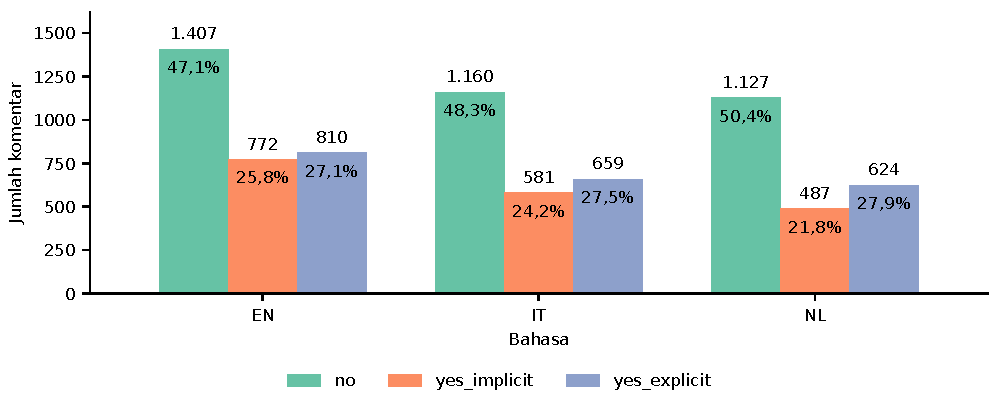
\includegraphics[width=\textwidth]{figures/eda_label_distribution.pdf}
\caption{Distribusi kelas sebelum pembagian. Jumlah komentar ditampilkan di atas batang dan persentase terhadap total per bahasa di dalam batang.}
\label{fig:eda-labels}
\end{figure*}

% Evidence: Q007.
Proporsi \texttt{no} mendekati separuh data pada ketiga bahasa, sedangkan \texttt{yes\_implicit} berada pada kisaran 21,76\%--25,83\%. Data Belanda memiliki proporsi \texttt{yes\_implicit} paling kecil. Distribusi ini perlu diperhatikan saat membaca hasil per kelas, tetapi belum cukup untuk menyimpulkan penyebab perbedaan kinerja antarbahasa. Distribusi label dan kemampuan mengenali setiap kelas dinilai secara terpisah.

\subsection{Prapemrosesan dan Pembagian Data}
% Evidence: Q005,Q007,B002.
Pemeriksaan tidak menemukan nilai kosong pada kolom yang dianalisis. Seluruh ID unik dan label sesuai tiga kelas. Satu duplikasi komentar pada data Italia memiliki label yang sama dan berada pada \textit{train}. Seluruh komentar tetap teralokasi tanpa perubahan isi. Tidak ditemukan tumpang tindih ID, komentar ternormalisasi, atau pasangan judul--deskripsi nonkosong antarbagian. Jumlah hasil pembagian disajikan pada Tabel~\ref{tab:split}.

% Evidence: Q005,Q007.
Hasil pembagian mendekati target 70:10:20, dengan jumlah aktual mengikuti kelompok komentar yang dipertahankan bersama. Dengan demikian, rasio tidak dipaksakan tepat apabila memerlukan pemisahan anggota kelompok. Pemeriksaan tumpang tindih membantu memastikan bahwa komentar yang sama tidak muncul pada bagian yang digunakan untuk pelatihan dan pengujian.

\begin{table}[t]
\centering\small
\begin{tabular}{lrrr}
\toprule
Data & \textit{Train} & \textit{Validation} & \textit{Test} \\
\midrule
EN & 2.111 & 292 & 586 \\
IT & 1.699 & 220 & 481 \\
NL & 1.556 & 226 & 456 \\
\bottomrule
\end{tabular}
\caption{Jumlah komentar setelah pembagian. Ketiga kelas hadir pada setiap bagian.}
\label{tab:split}
\end{table}

\subsection{Hasil Klasifikasi Berdasarkan Bahasa}
% Evidence: Q002,B002.
Seluruh pilihan \textit{prompt} Qwen memperoleh \textit{macro-F1} lebih tinggi daripada XLM-R, seperti ditunjukkan pada Tabel~\ref{tab:main}. Pada data Inggris, skor tertinggi diperoleh dengan \textit{prompt} Inggris. Pada data Italia, skor tertinggi juga diperoleh dengan \textit{prompt} Inggris, sedangkan pada data Belanda dengan \textit{prompt} Belanda. Kesamaan bahasa \textit{prompt} dan komentar belum memberikan hasil tertinggi secara konsisten.

\begin{table}[t]
\centering\small
\setlength{\tabcolsep}{2pt}
\begin{tabular}{lrrrr}
\toprule
Data & XLM-R & Q-EN & Q-IT & Q-NL \\
\midrule
EN & 0.529052 & \textbf{0.719146} & 0.715757 & 0.688340 \\
IT & 0.574515 & \textbf{0.7036} & 0.694249 & 0.701449 \\
NL & 0.507678 & 0.629927 & 0.630810 & \textbf{0.641522} \\
\bottomrule

\end{tabular}
\caption{\textit{Macro-F1} pada \textit{test}. Q-EN, Q-IT, dan Q-NL adalah Qwen dengan bahasa \textit{prompt} EN, IT, dan NL. Nilai Qwen tertinggi per bahasa dicetak tebal.}
\label{tab:main}
\end{table}

\begin{table*}[t]
\centering\small
\begin{tabular}{lllrrr}
\toprule
Data & Model & \textit{Prompt} & \texttt{no} & \texttt{yes\_implicit} & \texttt{yes\_explicit} \\
\midrule
EN & XLM-R & -- & 0.6569 & 0.4085 & 0.5217 \\
EN & Qwen & EN & \textbf{0.8406} & \textbf{0.6172} & 0.6996 \\
EN & Qwen & IT & 0.8229 & 0.5882 & \textbf{0.7362} \\
EN & Qwen & NL & 0.8250 & 0.5397 & 0.7003 \\
IT & XLM-R & -- & 0.7056 & 0.4747 & 0.5432 \\
IT & Qwen & EN & \textbf{0.7876} & \textbf{0.6127} & 0.7104 \\
IT & Qwen & IT & 0.7786 & 0.5815 & \textbf{0.7227} \\
IT & Qwen & NL & 0.7806 & 0.6020 & 0.7217 \\
NL & XLM-R & -- & 0.6742 & 0.3304 & 0.5185 \\
NL & Qwen & EN & 0.8118 & \textbf{0.5094} & 0.5686 \\
NL & Qwen & IT & 0.7908 & 0.4806 & 0.6210 \\
NL & Qwen & NL & \textbf{0.8140} & 0.4828 & \textbf{0.6278} \\
\bottomrule

\end{tabular}
\caption{F1 setiap kelas pada \textit{test}. Kolom \textit{prompt} hanya berlaku untuk Qwen. Nilai Qwen tertinggi pada setiap kelas dan bahasa data dicetak tebal.}
\label{tab:classes}
\end{table*}

% Evidence: Q002,B002.
Selisih skor Qwen tertinggi dan terendah adalah sekitar 0,0308 pada data Inggris, 0,0094 pada data Italia, dan 0,0116 pada data Belanda. Seluruh pilihan \textit{prompt} menghasilkan skor lebih rendah pada data Belanda dibandingkan dua bahasa lain. Hasil tertinggi ini bersifat deskriptif, bukan pengaturan akhir yang dipilih berdasarkan \textit{validation}. Perbedaan ukuran model, \textit{tokenizer}, batas \textit{input}, dan pelatihan juga membuat selisih XLM-R dan Qwen belum dapat dikaitkan dengan satu komponen tertentu.

% Evidence: Q002,B002.
Jika dibandingkan dengan skor Qwen tertinggi yang teramati, selisih terhadap XLM-R adalah sekitar 0,1901 pada data Inggris, 0,1291 pada data Italia, dan 0,1338 pada data Belanda. Hasil tersebut mendukung penggunaan Qwen yang disesuaikan dengan data berlabel sebagai pendekatan penyelesaian pada pembagian internal ini. Namun, skor tunggal belum menunjukkan kestabilan keunggulan tersebut pada pembagian atau pengulangan lain.

\subsection{Analisis Berdasarkan Kelas}
% Evidence: Q002,B002.
Tabel~\ref{tab:classes} memperlihatkan bahwa \texttt{no} memperoleh F1 tertinggi dan \texttt{yes\_implicit} terendah pada setiap pengaturan kedua model. Seluruh pilihan \textit{prompt} Qwen menghasilkan F1 lebih tinggi daripada XLM-R untuk ketiga kelas pada bahasa data yang sama.



% Evidence: Q002.
Pada data Inggris dan Italia, \textit{prompt} Inggris memberikan F1 tertinggi untuk \texttt{no} dan \nolinkurl{yes_implicit}, sedangkan \textit{prompt} Italia tertinggi untuk \nolinkurl{yes_explicit}. Pada data Belanda, \textit{prompt} Belanda tertinggi untuk \texttt{no} dan \nolinkurl{yes_explicit}, tetapi \textit{prompt} Inggris tertinggi untuk \nolinkurl{yes_implicit}. Dengan demikian, \textit{prompt} dengan \textit{macro-F1} tertinggi belum tentu terbaik pada setiap kelas.

% Evidence: Q002.
Pada kelas \texttt{yes\_implicit}, F1 Qwen berada pada rentang 0,5397--0,6172 untuk data Inggris, 0,5815--0,6127 untuk data Italia, dan 0,4806--0,5094 untuk data Belanda. Bahkan pilihan \textit{prompt} tertinggi pada kelas tersebut masih menghasilkan skor lebih rendah daripada dua kelas lainnya dalam pengaturan yang sama. Perbaikan klasifikasi perlu memberi perhatian pada pembedaan kategori ini, dengan pemeriksaan contoh prediksi untuk mengetahui bentuk kesalahan yang terjadi.

\section{Kesimpulan}
% Evidence: Q001,Q002,Q004,B002.
Penyelesaian Subtask B StereoQueerEval menggunakan SFT LoRA pada Qwen3.5-9B menghasilkan skor lebih tinggi daripada XLM-R pada pengujian internal. Skor tertinggi adalah 0,719146 pada data Inggris, 0,7036 pada data Italia, dan 0,641522 pada data Belanda. Kesamaan bahasa \textit{prompt} dan komentar belum konsisten memberikan hasil tertinggi. Pengembangan berikutnya perlu memperkuat klasifikasi \texttt{yes\_implicit} dan memilih pengaturan melalui \textit{validation}.

\section*{Keterbatasan}
% Evidence: Q001,Q004,Q006,Q008,B002,L119.
Percobaan menggunakan satu \textit{seed} dan satu versi \textit{prompt} per bahasa. Setiap pasangan Qwen melatih \textit{adapter} terpisah, sehingga hasil tidak mengisolasi perbedaan bahasa \textit{prompt} pada satu model terlatih. Variasi antarpengulangan belum diukur. Kesamaan \textit{seed} juga belum menjamin hasil identik lintas versi perangkat lunak atau GPU \citep{pytorch-reproducibility}. Reproduksi Qwen memerlukan kesamaan model dasar, \textit{tokenizer}, \textit{prompt}, pembagian data, dan konfigurasi pelatihan, dengan kebutuhan komputasi yang membatasi pengulangan pada perangkat lebih kecil.

% Evidence: Q001,Q004,Q008,L119.
Pengulangan dengan beberapa \textit{seed} dan pelaporan rata-rata beserta variasi skor diperlukan untuk menilai reproduksibilitas Qwen. Selain konfigurasi pelatihan, versi model dasar dan perangkat lunak perlu dipertahankan agar perbandingan antarpengulangan dapat ditafsirkan dengan lebih jelas.

% Evidence: Q005,Q007,L110.
Hasil belum menggambarkan kinerja pada \textit{test} resmi atau platform lain. Pasangan judul--deskripsi hanya menjadi pendekatan identitas video saat pembagian. Penyebab kesalahan pada masing-masing komentar masih memerlukan pemeriksaan langsung terhadap prediksi.

\bibliography{references}
\end{document}
